%%%%%%%%%%%%%%%%%%%%%%%%%%%%%%%%%%%
%This is the LaTeX ARTICLE template for RSC journals
%Copyright The Royal Society of Chemistry 2016
%%%%%%%%%%%%%%%%%%%%%%%%%%%%%%%%%%%

\documentclass[twoside,twocolumn,9pt]{article}
\usepackage{extsizes}
\usepackage[super,sort&compress,comma]{natbib}
\usepackage[version=3]{mhchem}
\usepackage[left=1.5cm, right=1.5cm, top=1.785cm, bottom=2.0cm]{geometry}
\usepackage{balance}
\usepackage{times,mathptmx}
\usepackage{sectsty}
\usepackage{graphicx}
\usepackage{lastpage}
\usepackage[format=plain,justification=justified,singlelinecheck=false,font={stretch=1.125,small,sf},labelfont=bf,labelsep=space]{caption}
\usepackage{float}
\usepackage{fancyhdr}
\usepackage{fnpos}
\usepackage[english]{babel}
\usepackage{amsmath}
\addto{\captionsenglish}{%
  \renewcommand{\refname}{Notes and references}
}
\usepackage{array}
\usepackage{droidsans}
\usepackage{charter}
\usepackage[T1]{fontenc}
\usepackage[usenames,dvipsnames]{xcolor}
\usepackage{setspace}
\usepackage[compact]{titlesec}
\usepackage{hyperref}
%%%Please don't disable any packages in the preamble, as this may cause the template to display incorrectly.%%%

\newcommand*{\citen}[1]{%
	\begingroup
	\romannumeral-`\x % remove space at the beginning of \setcitestyle
	\setcitestyle{numbers}%
	\cite{#1}%
	\endgroup
}

\usepackage{epstopdf}%This line makes .eps figures into .pdf - please comment out if not required.

\definecolor{cream}{RGB}{222,217,201}

\begin{document}

\pagestyle{fancy}
\thispagestyle{plain}
\fancypagestyle{plain}{

%%%HEADER%%%
\fancyhead[C]{
\includegraphics[width=18.5cm]{head_foot/header_bar}}
\fancyhead[L]{\hspace{0cm}\vspace{1.5cm}
\includegraphics[height=30pt]{head_foot/journal_name}}
\fancyhead[R]{\hspace{0cm}\vspace{1.7cm}
\includegraphics[height=55pt]{head_foot/RSC_LOGO_CMYK}}
\renewcommand{\headrulewidth}{0pt}
}
%%%END OF HEADER%%%

%%%PAGE SETUP - Please do not change any commands within this section%%%
\makeFNbottom
\makeatletter
\renewcommand\LARGE{\@setfontsize\LARGE{15pt}{17}}
\renewcommand\Large{\@setfontsize\Large{12pt}{14}}
\renewcommand\large{\@setfontsize\large{10pt}{12}}
\renewcommand\footnotesize{\@setfontsize\footnotesize{7pt}{10}}
\makeatother

\renewcommand{\thefootnote}{\fnsymbol{footnote}}
\renewcommand\footnoterule{\vspace*{1pt}%
\color{cream}\hrule width 3.5in height 0.4pt \color{black}\vspace*{5pt}}
\setcounter{secnumdepth}{5}

\makeatletter
\renewcommand\@biblabel[1]{#1}
\renewcommand\@makefntext[1]%
{\noindent\makebox[0pt][r]{\@thefnmark\,}#1}
\makeatother
\renewcommand{\figurename}{\small{Fig.}~}
\sectionfont{\sffamily\Large}
\subsectionfont{\normalsize}
\subsubsectionfont{\bf}
\setstretch{1.125} %In particular, please do not alter this line.
\setlength{\skip\footins}{0.8cm}
\setlength{\footnotesep}{0.25cm}
\setlength{\jot}{10pt}
\titlespacing*{\section}{0pt}{4pt}{4pt}
\titlespacing*{\subsection}{0pt}{15pt}{1pt}
%%%END OF PAGE SETUP%%%

%%%FOOTER%%%
\fancyfoot{}
\fancyfoot[LO,RE]{\vspace{-7.1pt}
\includegraphics[height=9pt]{head_foot/LF}}
\fancyfoot[CO]{\vspace{-7.1pt}\hspace{13.2cm}
\includegraphics{head_foot/RF}}
\fancyfoot[CE]{\vspace{-7.2pt}\hspace{-14.2cm}
\includegraphics{head_foot/RF}}
\fancyfoot[RO]{\footnotesize{\sffamily{1--\pageref{LastPage} ~\textbar  \hspace{2pt}\thepage}}}
\fancyfoot[LE]{\footnotesize{\sffamily{\thepage~\textbar\hspace{3.45cm} 1--\pageref{LastPage}}}}
\fancyhead{}
\renewcommand{\headrulewidth}{0pt}
\renewcommand{\footrulewidth}{0pt}
\setlength{\arrayrulewidth}{1pt}
\setlength{\columnsep}{6.5mm}
\setlength\bibsep{1pt}
%%%END OF FOOTER%%%

%%%FIGURE SETUP - please do not change any commands within this section%%%
\makeatletter
\newlength{\figrulesep}
\setlength{\figrulesep}{0.5\textfloatsep}

\newcommand{\topfigrule}{\vspace*{-1pt}%
\noindent{\color{cream}\rule[-\figrulesep]{\columnwidth}{1.5pt}} }

\newcommand{\botfigrule}{\vspace*{-2pt}%
\noindent{\color{cream}\rule[\figrulesep]{\columnwidth}{1.5pt}} }

\newcommand{\dblfigrule}{\vspace*{-1pt}%
\noindent{\color{cream}\rule[-\figrulesep]{\textwidth}{1.5pt}} }

\makeatother
%%%END OF FIGURE SETUP%%%

%%%TITLE, AUTHORS AND ABSTRACT%%%
\twocolumn[
  \begin{@twocolumnfalse}
\vspace{3cm}
\sffamily
\begin{tabular}{m{4.5cm} p{13.5cm} }


\includegraphics{head_foot/DOI} & \noindent\LARGE{\textbf{Bayesian determination of the effect of a deep eutectic solvent on the structure of lipid monolayers}} \\%Article title goes here instead of the text "This is the title"
\vspace{0.3cm} & \vspace{0.3cm} \\

 & \noindent\large{Andrew R. McCluskey,\textit{$^{ab}$}$^{\ddag}$ Adrian Sanchez-Fernandez,\textit{$^{ac}$}$^{\ddag\P}$ Karen J. Edler,\textit{$^{a}$}$^{\ast}$ Stephen C. Parker,\textit{$^{a}$} Andrew J. Jackson,\textit{$^{cd}$} Richard A. Campbell,\textit{$^{ef}$} and Thomas Arnold\textit{$^{abcg}$}$^{\ast}$} \\%Author names go here instead of "Full name", etc.


\includegraphics{head_foot/dates} & \noindent\normalsize{Deep eutectic solvents present a novel class of non-aqueous room temperature solvent with tunable properties, that are capable of promoting the self-assembly of surfactant molecules. However, the solvation model in these systems still challenges the classic understanding of amphiphilicity. In this work, we present the first example of the self-assembly of phospholipid monolayers at the interface between air and a non-aqueous solvent. Furthermore, we use novel, chemically-consistant Bayesian modelling of X-ray and neutron reflectometry measurements to show the ability of the deep eutectic solvent to interact with the phosphatidylglycerol lipid head component, leading to an apparent increase in the component volume compared to that observed in water. No such change was observed for the phosphocholine head component, indicating that the interaction is head component specific.} \\

\end{tabular}

	\end{@twocolumnfalse} \vspace{0.6cm}

  ]
%%%END OF TITLE, AUTHORS AND ABSTRACT%%%

%%%FONT SETUP - please do not change any commands within this section
\renewcommand*\rmdefault{bch}\normalfont\upshape
\rmfamily
\section*{}
\vspace{-1cm}


%%%FOOTNOTES%%%

\footnotetext{\textit{$^{a}$~Department of Chemistry, University of Bath, Claverton Down, Bath, BA2 7AY, UK.}}
\footnotetext{\textit{$^{b}$~Diamond Light Source, Harwell Campus, Didcot, OX11 0DE, UK.}}
\footnotetext{\textit{$^{c}$~European Spallation Source, SE-211 00 Lund, Sweden.}}
\footnotetext{\textit{$^{d}$~Department of Physical Chemistry, Lund University, SE-211 00 Lund, Sweden.}}
\footnotetext{\textit{$^{e}$~Institut Laue-Langevin, 71 avenue des Martyrs, 38000, Grenoble, France.}}
\footnotetext{\textit{$^{f}$~Division of Pharmacy and Optometry, University of Manchester, Manchester, M13 9PT, UK.}}
\footnotetext{\textit{$^{g}$~ISIS Neutron and Muon Source, Science and Technology Facilities Council, Rutherford Appleton Laboratory, Harwell Oxford, Didcot OX11 0QX, UK.}}
\footnotetext{\textit{$^{\P}$~Present address: Department of Food Technology, Lund University, SE-211 00 Lund, Sweden}}
\footnotetext{$^{\ast}$~Corresponding author: k.edler@bath.ac.uk, tom.arnold@esss.se}


%Please use \dag to cite the ESI in the main text of the article.
%If you article does not have ESI please remove the the \dag symbol from the title and the footnotetext below.
\footnotetext{\dag~Electronic Supplementary Information (ESI) available: All datasets, figure file and analysis/plotting scripts, allowing for a fully reproducible analysis of all work presented herein. See DOI: 10.6084/m9.figshare.6661784}
%additional addresses can be cited as above using the lower-case letters, c, d, e... If all authors are from the same address, no letter is required

\footnotetext{$^{\ddag}$~These authors have contributed equally to the work presented within.}
%\footnotetext{\ddag~Additional footnotes to the title and authors can be included \textit{e.g.}\ `Present address:' or `These authors contributed equally to this work' as above using the symbols: \ddag, \textsection, and \P. Please place the appropriate symbol next to the author's name and include a \texttt{\textbackslash footnotetext} entry in the the correct place in the list.}


%%%END OF FOOTNOTES%%%

%%%MAIN TEXT%%%%
\section{Introduction}
Deep eutectic solvents (DES) are green, sustainable solvents obtained through the complexation of naturally occurring compounds, such as sugars, alcohols, amines and carboxylic acids, among others.\cite{Smith2014, Dai2013} An extensive hydrogen-bonding network is present between these precursors, allowing the mixture to remain liquid at room temperature.\cite{Hammond2016, Hammond2017, Araujo2017} Additionally, through different combinations of the precursor materials, it is possible to tune the physicochemical properties of the solvent, such as polarity,\cite{Pandey2014} viscosity and surface tension,\cite{Smith2014} network charge,\cite{Zahn2016} and hydrophobicity.\cite{Ribeiro2015,vanOsch2015}

It has recently been shown that these solvents have the ability to promote the self-assembly of surfactants into micellar structures\cite{Sanchez-Fernandez2016,Arnold2015} and to stabilise the conformation of non-ionic polymer species,\cite{Sapir2016} indicating the presense of a solvophobic effect. The behaviour and conformation of biomolecules in DES have seen an increase in interest,\cite{Esquembre2013,Gorke2010,Gorke2008,Monhami2014,Wu2014,Harifi-Mood2017,Milano2017,Sanchez-Fernandez2017} due to potential application in the preservation of biomolecules as environments for enzymatic reactions.\cite{Merza2018} Futhermore, recent investigations have also shown that DES have been able to support the formation of phospholipid bilayers.\cite{Bryant2017,Bryant2016,Gutierrez2009}

The formation of phospholipid monolayers at the air/liquid interface also plays a key role in many biological and technological processes. The solvent-specific solubility of different components of the phospholipid results in the formation of a stable monolayer of phospholipid at the interface.\cite{Mohwald1990} Phospholipids contain a charged head, either anionic or zwitterionic, and investigations at the air-salt water interface have revealed the importance of the phospholipid-ion interactions on structure, monomer packing, and stability of the monolayer.\cite{Mohwald1990,Kewalramani2010} Despite the broad interest in these systems, the presence of stable phospholipid monolayers at the interface between air and a non-aqueous media has not been previously reported, to the best of the authors' knowledge.

Recent developments in computational resources and software have enabled powerful methodologies and algorithms to be harnessed by those from non-expert backgrounds. This has benefitted significantly from open-source software projects such as the Python language\cite{vanRossum1995} and the Jupyter notebooks framework.\cite{Kluyver2016} In the area of neutron and X-ray reflectometry data-analysis, the landscape of open-source software is diverse, with a range of software packages available from a variety of sources; refnx\cite{Nelson2018}, motofit,\cite{Nelson2006} Aurore,\cite{Gerelli2016} and GenX.\cite{Bjorck2007} The Python library refnx is particularly powerful due to the ability to implement complete custom models which can contain chemically-relevant information.

The use of a Python library for fitting enables powerful probability distribution function (PDF) sampling methods to be used such as the Goodman \& Weare Affine Invariant Markov chain Monte Carlo (MCMC) Ensemble,\cite{Goodman2010} as implemented in the Python library emcee.\cite{Foreman-Mackey2013} This is a method for sampling a high-dimensionality parameter space, such as that which is relevant in reflectometry fitting, in a Bayesian fashion, where the new samples are generated with consideration of those sampled previously. The use of Bayesian inference allows the PDF for each fitting variable to be probed, therefore estimations of the inverse uncertainties associated with each parameter can be found as well as information about the correlations between different variables.

In this work, we present the first investigation of the structure of phospholipid monolayers at the air-DES interface, as determined by chemically-consistant modelling of X-ray reflectometry (XRR) measurements. Four different phospholipids; 1,2-dipalmitoyl-sn-glycero-3-phosphocholine (DPPC), 1,2-dimyristoyl-sn-glycero-3-phosphocholine (DMPC),  1,2-dilauroyl-sn-glycero-3-phosphocholine (DLPC) and 1,2-dimyristoyl-sn-glycero-3-phospho-(1'-rac-glycerol) (DMPG), were studied at the interface between a 1:2 mixture of choline chloride:glycerol and air. This allowed the nature of two, chemically distinct, phospholipid head components to be understood in this non-aqueous solvent, in addition to the effect of the tail chain length. The analysis was then extended to model complementary neutron reflectometry measurements for two contrasts of DMPC and DPPC at a single surface pressure.

\section{Experimental}

\subsection{Materials}
Choline chloride (99 \%, Sigma-Aldrich) and glycerol (99 \%, Sigma-Aldrich) d$_9$-choline chloride (99 \%, 98 \% D, CK Isotopes) and d$_8$-glycerol (99 \%, 98 \% D, CK Isotopes)  were purchased and used without further purification. The DES was prepared by mixing the precursors at the appropriate ratio, and heating at 80 $^\circ$C until a homogeneous, transparent liquid formed.\cite{Smith2014} The solvent was equilibrated overnight at 40 $^\circ$C and subsequently stored under a dry atmosphere. Due to the limited availability of the deuterated precursors, a fully protonated subphase (hDES) and a partially deuterated subphase (hdDES) were prepared and used during the neutron reflectometry (NR) experiment. The partially deuterated subphase was prepared using the following mixtures of precursors: 1 mole of 0.38 fraction of h-choline chloride/0.62 mole fraction of d-choline chloride; and 2 moles of 0.56 mole fraction of h-glycerol/0.44 mole fraction of d-glycerol. The solvent was subsequently prepared following the procedure discussed above.

The water content of the DES was determined before and after each experiment by Karl-Fischer titration (Mettler Toledo DL32 Karl-Fischer Coulometer, Aqualine Electrolyte A, Aqualine Catholyte CG A) in order to ensure water presence was kept to a minimum. Those measurements showed that the water content of the solvent was kept below 0.3 wt\% during all the experimental procedures presented here, which we assume to be negligible and have little impact on the characteristics of the DES.\cite{Hammond2016,Hammond2017}

DPPC (> 99 \%, C$_{16}$ tails), DMPC (> 99 \%, C$_{14}$ tails), and DMPG (> 99 \%, C$_{14}$ tails) were supplied by Avanti Polar Lipids and DLPC (> 99 \%, C$_{12}$ tails) was supplied by Sigma-Aldrich and all were used as received. Deuterated versions of DPPC (d$_{62}$-DPPC, > 99 \%, deuterated tails-only) and DMPC (d$_{54}$-DPPC, > 99 \%, deuterated tails-only) were supplied by Avanti Polar Lipids and used without further purification. These phospholipids were dissolved in chloroform (0.5 mg/mL) at room temperature. PC indicates the molcule contains a phosphocholine head component, where PG contains a phosphoditylglycerol head component, these are shown in Figure \ref{fig:heads}.

\begin{figure}
	\centering
	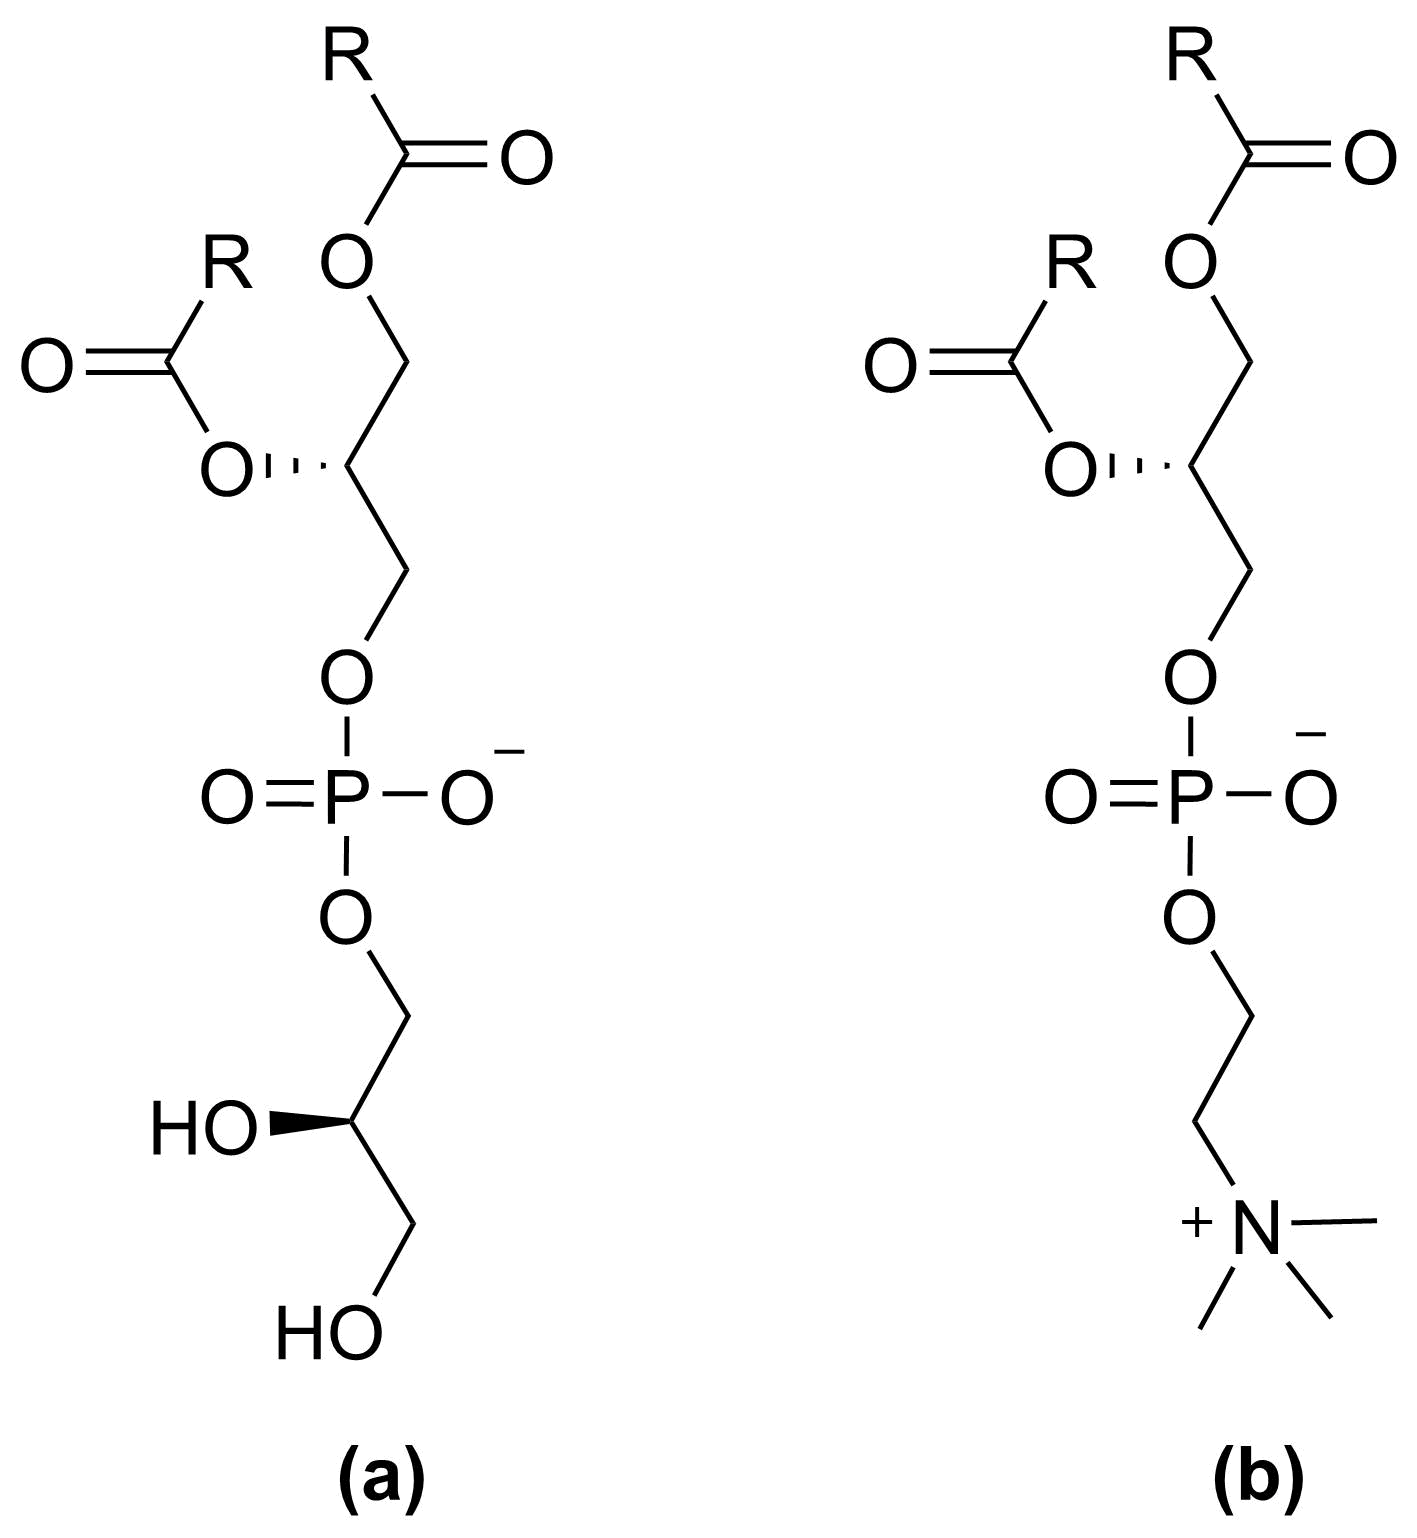
\includegraphics[width=0.30\textwidth]{figures/head_groups}
	\caption{The two lipid classes with different head components compared in this study, where R indicates the hydrocarbon tail; (a) phosphatidylglycerol, (b) phosphocholine. Source: Datasets, figure files and running/plotting scripts are available under CC-BY.\cite{mccluskey_2018}}
	\label{fig:heads}
\end{figure}

\begin{table*}
	\small
	\caption{\ Lipid component volumes extracted from different literature sources. $V_l$ corresponds to the total lipid volume, MD to molecular dynamics simulation, WAXS to wide-angle X-ray scattering, NB to neutral buoyancy and DVTD to differential vibrating tube densimetry. $^a$ The values for the head component in Kucerka \emph{et al.},\cite{Kucerka2004} were taken from Balgav\'{y} \emph{et al}.\cite{Balgavy2001}}
	\label{tab:water}
	\begin{tabular*}{\textwidth}{@{\extracolsep{\fill}}llllllllll}
		\hline
    Lipid & DPPC & & & DMPC & & DLPC & & DMPG & POPG \\
    \hline
    Reference & [\citen{Armen1998}] & [\citen{Sun1994}] & [\citen{Kucerka2004,Balgavy2001}]$^a$ & [\citen{Armen1998}] & [\citen{Kucerka2004,Balgavy2001}]$^a$ & [\citen{Armen1998}] & [\citen{Kucerka2004,Balgavy2001}]$^a$ & [\citen{Pan2012}] & [\citen{Kucerka2012}] \\
    \hline
    $V_l$/\AA$^3$ & $1287.3\pm25.5$ & $1148\pm2$ & $1264.2\pm32.1$ & $1172.5\pm25.1£$ & $1155.4\pm30.0£$ & $1057.7\pm24.7$ & $1046.6\pm28.0$ & $1011.4$ & $1203$ \\
    $V_t$/\AA$^3$ & $966.4\pm5.4$ & $829\pm4$ & $924.7\pm17.6$ & $851.5\pm5.0£$ & $815.9\pm15.5£$ & $736.8\pm4.6$ & $707.1\pm13.5$ & $720.4$ & $914$ \\
    $V_h$/\AA$^3$ & $320.9\pm20.1$ & $319\pm6$ & $339.5\pm14.5$ & $320.9\pm20.1$ & $339.5\pm14.5$ & $320.9\pm20.1$ & $339.5\pm14.5$ & $291.0$ & $289$ \\
    Method & MD & WAXS & NB & MD & NB & MD & NB & DVTD & MD \\
    T/$^\circ$C & 50 & 24 & 30 & 50 & 30 & 50 & 30 & 20 & 25 \\
	\end{tabular*}
\end{table*}
In the XRR experiment, sample preparation was performed in situ using the standard method for the spreading of insoluble monolayers on water: a certain amount of the phospholipid solution was spread onto the liquid surface in order to provide a given surface concentration. After the evaporation of the chloroform, it is assumed that the resulting system is a solvent subphase with a monolayer of phospholipid at the interface. Surface concentration was modified by closing and opening the PTFE barriers of a Langmuir trough. In order to minimise the volumes used in the NR experiment (to keep the cost of deuterated compounds to a manageable level) it was not possible to use a Langmuir trough. Instead, small Delrin adsorption troughs were used that did not have controlable barriers. So, although the surface coverage was nominally the same as used in the X-ray studies, the lack of precise control over the surface pressure meant that it was not appropriate to co-refine XRR and NR contrasts together.

\subsection{Methods}
XRR measurements were taken on I07 at Diamond Light Source, at 12.5 keV photon energy using the double-crystal-deflector.\cite{Arnold2012} The reflected intensity was measured in a momentum transfer range from 0.018 to 0.7 \AA$^{-1}$. The data were normalised with respect to the incident beam and the background was measured from off-specular reflection and subsequently subtracted. Samples were equilibrated for at least one hour and preserved under an argon atmosphere to minimise the adsorption of water by the subphase. XRR data were collected for each of the lipids, DLPC, DMPC, DPPC and DMPG at four surface pressures (DLPC: 20, 25, 30, and 35 mNm$^{-1}$, DMPC: 20, 25, 30, and 40 mNm$^{-1}$, DPPC: 15, 20, 25, and 30 mNm$^{-1}$, DMPG: 15, 20, 25, and 30 mNm$^{-1}$), as measured with an aluminium Wilhelmy plate; all measurements were conducted at 22 $^\circ$C. The aluminium Wilhelmy plate was used over a traditional paper plate due to the low wetability of paper by the DES.

The NR experiments were performed on FIGARO at the Institut Laue-Langevin using the time-of-flight method.\cite{Campbell2011} Data at two incident angles of 0.62$^\circ$ and 3.8$^\circ$ were measured to provide a momentum transfer range from 0.005 to 0.18 \AA$^{-1}$. Two surface pressures for each system and contrast was measured (DMPC: 20 and 25 mNm$^{-1}$, DPPC: 15 and 20 mNm$^{-1}$). Similar to the X-ray procedure, samples were given enough time to equilibrate (at least two hours), kept under an inert atmosphere, and all measurements were conducted at 22 $^\circ$C.

\subsection{Data analysis}
The use of XRR and NR to analyse the structure of phospholipids on the surface of water has a history extending over many years.\cite{Mohwald1990,Kewalramani2010,Bayerl1990,Johnson1991,Clifton2012,Helm1987,Daillant1990} The models used in the rationalisation of XRR and NR data have varied significantly in number of layers present, use of interfacial roughness, and parameterisation of physical constraints. Frequently these physical constraints include the component volumes of the phospholipid head and tail components, using values taken from other techniques, such as those shown in Table \ref{tab:water}. Additionally, a recent evaluation of the applicability of different models to surfactant and phospholipid monolayers from the NR perspective has been published,\cite{Campbell2018} suggests possible oversights in the modelling of NR data.

In Table \ref{tab:water}, there appears to be a general consensus that the component volume of the phosphocholine (PC) head is in the range from 320-360 \AA$^3$ while the phosphatidylglycerol (PG) head is in the range 289-291 \AA$^3$. However, we do not know whether the head component volumes used in the literature, that are derived from water-based measurements, will be appropriate for this work, which involves a non-aqueous solvent. The charged nature of the zwitterionic and anionic lipid heads means that they are likely to have different interactions with polar, but neutral, water as compared to the charged DES.\cite{Sanchez-Fernandez2018} Furthermore, it has been shown that in the liquid expanded and condensed phases, which are often present at high surface pressure, the lipid tails will become compressed resulting in a component volume less than measured from other techniques,\cite{Marsh2010,Small1984} and the need to take into account the compaction of the hydrocarbon chains of phospholipid monolayers according to their phase in the modelling of NR data has recently been demonstrated.\cite{Campbell2018}

In this work we would therefore like to use a model that does not assume the molecular volume while remaining physical meaningful. To do this we have allowed the lipid component volumes to vary while constraining the overall system to be self-consistent across multiple different measurements. To do this we have used the Python library refnx\cite{Nelson2018}. This software allows the inclusion of a custom model to be defined, from which parameters feed into the Abel\`{e}s reflectivity model (a model that is widely used to calculate reflectivity \cite{Abeles1950,Parratt1954}). This custom model, along with a series of Jupyter notebooks showing, in full, the analysis performed, can be found in the ESI and is available under CC-BY.\cite{mccluskey_2018}

Our chemically-consistent model is made up of two layers to define the lipid monolayer; the head layer at the interface with the solvent and tail layer at the interface with the air. The head components have a calculated scattering length, $b_h$, (found as a summation of the X-ray or neutron atomic scattering lengths), and a component volume, $V_h$. These head components make up a layer with a given thickness, $d_h$, and roughness, $\sigma_h$, within which some volume fraction of solvent can intercalate, $\phi_h$. The tail components also have a calculated scattering length, $b_t$, roughness, $\sigma_t$, and a component volume, $V_t$. We have defined the thickness of the tail layer, $d_t$, in terms of the maximum (all-trans) length of the carbon tail, $t_t$, and the angle that the chain is tilted by with respect to the interface normal, $\theta_t$,
%
\begin{equation}
\label{equ:tl}
d_t = t_t \cos{\theta_t}.
\end{equation}
%
This was used to impose a chemically-sensible maximum on the thickness of the lipid tail layer, e.g. it cannot be thicker than the maximum extended length of the lipid tail. The scattering length density (SLD) of the tail and head layers used in the Abel\`{e}s model can therefore be found as follows,
%
\begin{equation}
\text{SLD}_i = \frac{b_i}{V_i}(1 - \phi_i) + \text{SLD}_{s}(\phi_i),
\end{equation}
%
where, $\text{SLD}_{s}$ is the scattering length density of the subphase (DES), and $i$ indicates either the tail or head layer; it is assumed that the tail layer contains neither solvent nor air, e.g. $\phi_t = 0$. To ensure that the number density of head components and pairs of tail components is the same, the following constraint was included in the model,\cite{Braun2017}
%
\begin{equation}
\label{equ:phih}
\phi_h =  1 - \bigg(\frac{d_tV_h}{V_td_h}\bigg).
\end{equation}
%
Based on the work of Campbell \emph{et al.},\cite{Campbell2018} a single value for the interfacial roughness was fitted for all of the interfaces, including the subphase (i.e. $\sigma_h$ = $\sigma_t$ = $\sigma_s$), as there is only a single lipid molecule type in each monolayer. Therefore, any capillary wave roughness at the air-DES interface is carried equally through the layers.

In the first of two steps, this custom model was used to co-refine the component volume of the lipid head component, $V_h$, the volume of the tail component, $V_t$, and the head thickness, $d_h$ across XRR measurements at four different surface concentrations. The head thickness was not permitted to vary with surface pressure to reduce the dimensionality of the parameter space, an assumption that is based on our belief that increasing surface pressure should not significantly influence the head layer thickness. The following parameters were allowed to vary; $\theta_t$, and $\sigma_{t,h,s}$, independently across the surface pressures, while others, shown in Table \ref{tab:invariant}, were held constant at the values given. The length of the carbon chain was kept constant at the value determined by the Tanford equation,\cite{Tanford1980} since this is the maximum chain length possible and the most likely conformation at the surface pressures studied. For each co-refinement of four XRR measurements, there were, in total, eleven degrees of freedom in the fitting process. Throughout all of the analysis, the reflectometry scale factor was allowed to vary freely, while the background as constrained to the intensity of either the largest or second-largest $q$-value. 

%
\begin{table}[h]
	\small
	\caption{\ The invariant parameters within the chemically-consistent model.
	$^a$Values obtained from the Tanford formula.\cite{Tanford1980} $^b$Values obtained from Sanchez-Fernandez \emph{et al.}\cite{Sanchez-Fernandez2016}}
	\label{tab:invariant}
	\begin{tabular*}{0.48\textwidth}{@{\extracolsep{\fill}}lllll}
		\hline
		Component & $b_t$/fm & $b_h$/fm & $t_t$/\AA & $\text{SLD}$/$\times10^{-6}$\AA$^{-2}$ \\
		\hline
		X-ray & & & & \\
		DLPC & 5073 & 4674 & 15.5$^a$ & -- \\
		DMPC & 5985 & 4674 & 18.0$^a$ & -- \\
		DPPC & 6897 & 4674 & 20.5$^a$ & -- \\
		DMPG & 5985 & 4731 & 18.0$^a$ & --\\
		Air & -- & -- & -- & 0\\
		DES & -- & -- & -- & 10.8$^b$ \\
		\hline
		Neutron & & & & \\
		d$_{54}$-DMPC & 5329.8 & 602.7 & 18.0$^a$ & -- \\
		d$_{62}$-DPPC & 6129.2 & 602.7 & 20.5$^a$ & -- \\
		h-DES & -- & -- & -- & 0.43$^b$  \\
		hd-DES & -- & -- & -- & 3.15$^b$ \\
		\hline
	\end{tabular*}
\end{table}
%
In the second step, the head and tail component volumes, and head layer thickness determined from XRR were fixed for the refinement of the custom model against the NR measurements. This approach means that the number of variable parameters to fir the NR data can be reduced to two, namely the chain tilt angle, $\theta_t$, and the interfacial roughness, $\sigma_{t,h,s}$, for the co-refinement of two datasets. Table \ref{tab:invariant} also gives the details of the scattering lengths and SLDs used as invariant parameters for the NR fitting.

In both cases, the refinement of the custom model to the experimental data involved the transformation of the reflectometry calculated from the model and the data into $Rq^4$ such that the contribution of the Fresnel decay was removed, before using the differential evoluation method available to refnx from the scipy library,\cite{Jones2001} to find the parameters that gave the best fit to the data. The parameter space was then probed using the MCMC method available through emcee,\cite{Foreman-Mackey2013} which allowed for an estimate of the PDF associated with each parameter. In the MCMC sampling, 200 walkers were used over 1000 iterations, following an equilibration of 200 iterations. The use of MCMC sampling allowed for the Bayesian inference of the probability density function for each of the variables and their respective interactions (shown in detail in the ESI). This allowed asymmetric confidence intervals to be found for each of the variable parameters. However, it is important to note that these are not \emph{true} confidence intervals, and account only for the uncertainty present in the data, i.e. they do no account of systematic uncertainty in the measurement that are underrepresented, or unrepresented, in the experimental dataset.

%
\begin{figure}
	\centering
	
\includegraphics[width=0.48\textwidth]{figures/DLPC_all_data}
	
\includegraphics[width=0.48\textwidth]{figures/DMPC_all_data}
	
\includegraphics[width=0.48\textwidth]{figures/DPPC_all_data}
	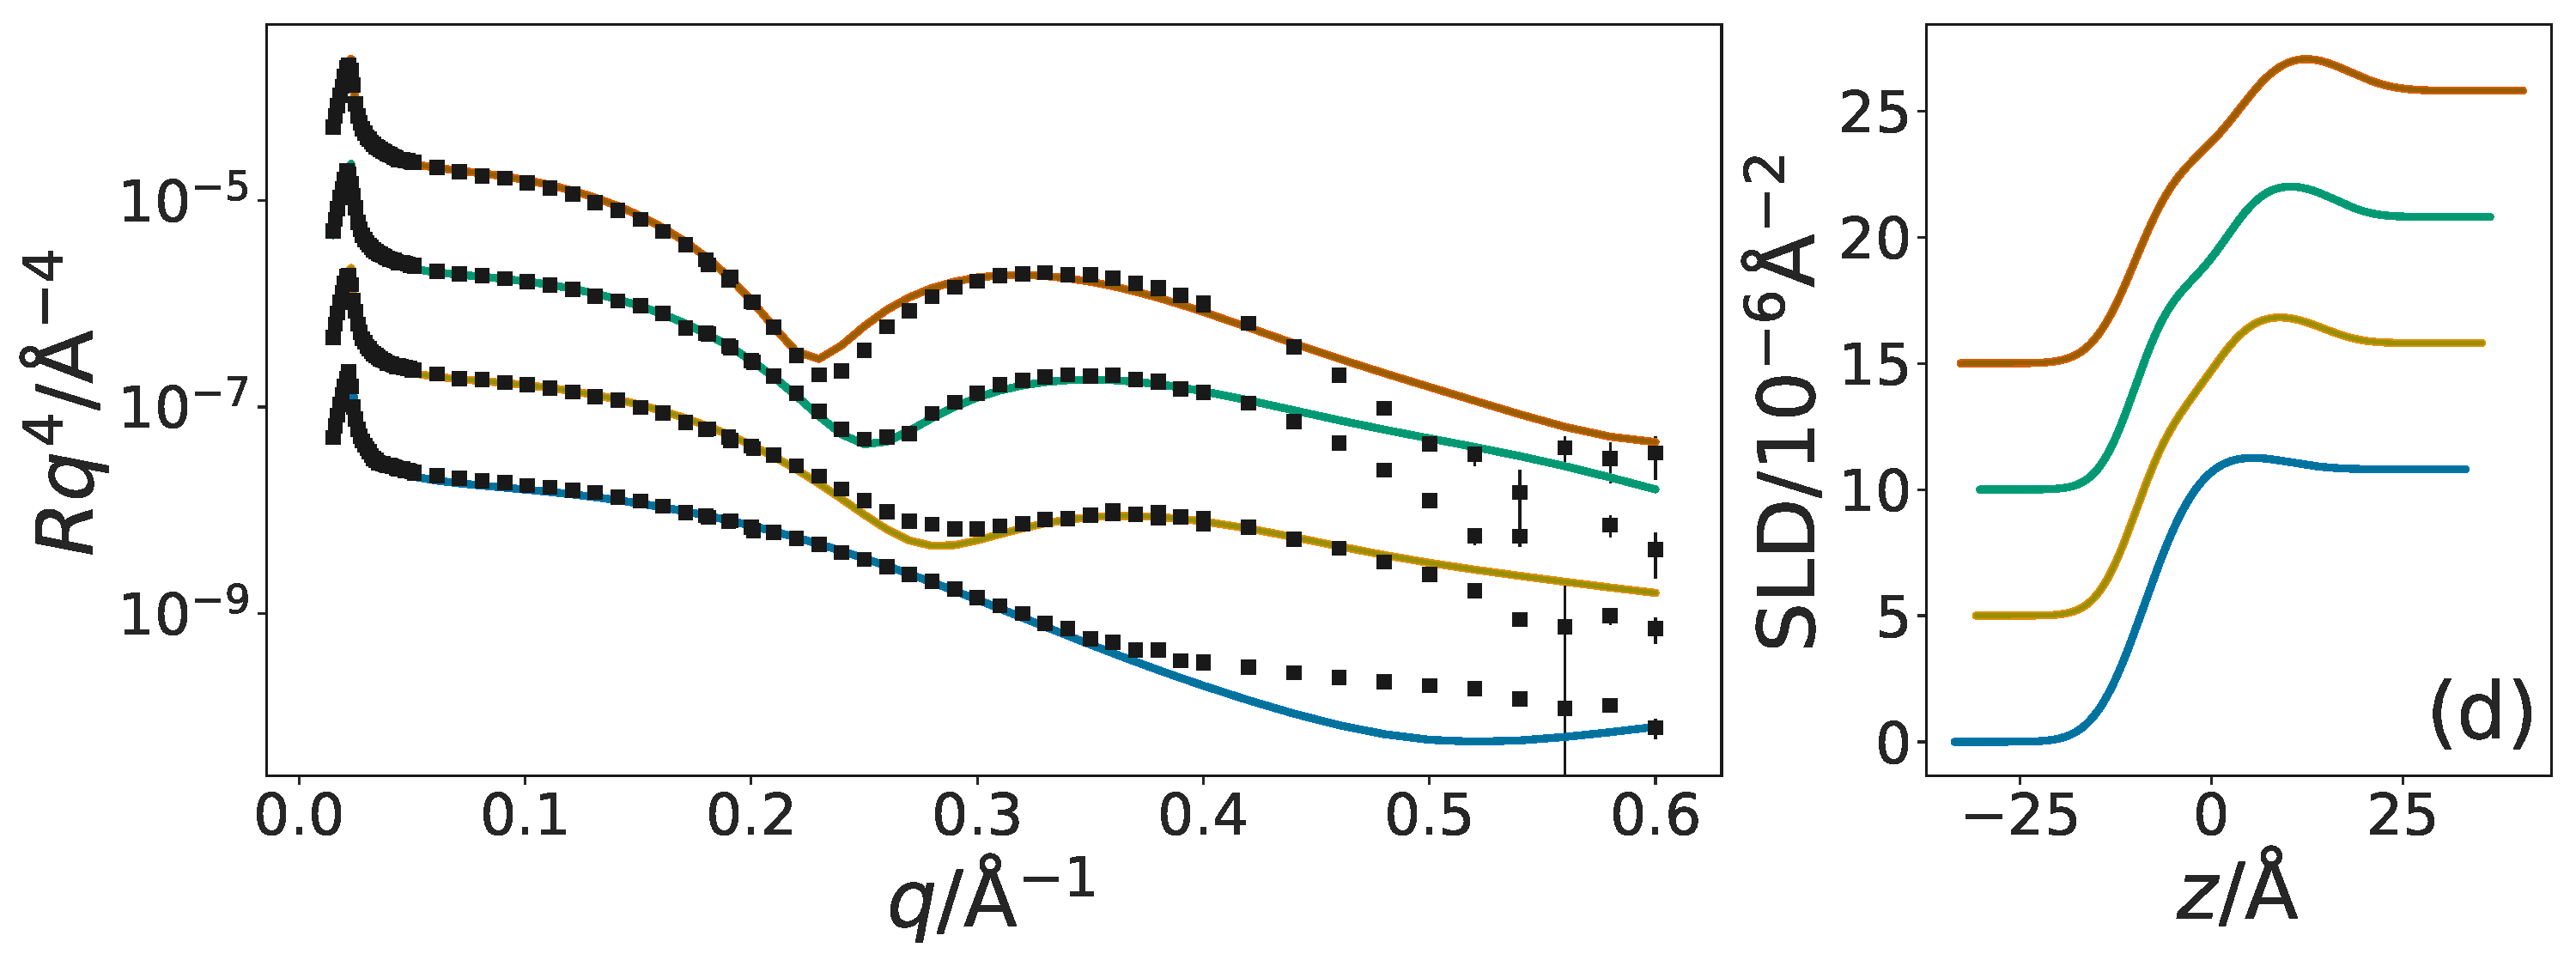
\includegraphics[width=0.48\textwidth]{figures/DMPG_all_data}
	\caption{The XRR profiles (left) and SLD profiles (right) for each of the four lipids; (a) DLPC, (b) DMPC, (c) DPPC, (d) DMPG, at the four measured surface pressures; lowest surface pressure at the bottom and increasing moving up. The different surface pressure XRR profiles have been offset in the $y$-axis by an order of magnitude and SLD profiles offset in the $y$-axis by $5\times10^{-6}$ \AA$^{-2}$, for clarity. Source: Datasets, figure files and running/plotting scripts are available under CC-BY.\cite{mccluskey_2018}}
	\label{fig:lipids}
\end{figure}
%
\section{Results \& Discussion}
The chemically-consistent model was co-refined across the four surface pressure XRR measurements for each lipid. The resulting XRR profiles, associated SLD profiles are shown in Figure \ref{fig:lipids}. Table \ref{tab:liptab} gives details of all varying parameters for each lipid at the highest surface pressure measured, as well as the details of the $d_t$ and $\phi_h$ which are determined from Eqns. \ref{equ:tl} and \ref{equ:phih} respectively, each value is given with asymmetric uncertainies that corresponds to a 95 \% confidence interval of the PDF; the full PDF plots can be found in the ESI.

The custom model was used to co-refine the two contrasts of NR measurements for each lipid, at each surface pressure. The resulting NR profiles and associated SLD profiles, at a surface pressure of 20 mNm$^{-1}$ are given in Figure \ref{fig:neutron}. Table \ref{tab:neutron} gives details of the varying parameters at each surface pressure as well as the details of the $d_t$ and $\phi_h$ which are determined from Eqns. \ref{equ:tl} and \ref{equ:phih} respectively; again these are given with a asymmetric uncertainties corresponding to a 95 \% confidence interval and the full PDF plots can be found in the ESI.
%
\begin{table}
	\small
	\caption{\ The best-fit values, and associated 95 \% confidence intervals for the varying parameters in the XRR models, at the highest surface pressure (SP) measured. The values of $d_t$ were found from the appropriate values of $\theta_t$ using Eqn. \ref{equ:tl} and the values for $\phi_h$ were obtained from the appropriate use of Eqn. \ref{equ:phih}}
	\label{tab:liptab}
	\begin{tabular*}{0.48\textwidth}{@{\extracolsep{\fill}}lllll}
		\hline
		Lipid & DLPC & DMPC & DPPC & DMPG \\
    SP/mNm$^{-1}$ & 35 & 40 & 30 & 30 \\
		\hline
		$\theta_t$/$^\circ$ & \input{../output/dlpc/angle35.txt} & \input{../output/dmpc/angle40.txt} & \input{../output/dppc/angle30.txt} & \input{../output/dmpg/angle30.txt} \\
		$\sigma_{t,h,s}$/\AA & \input{../output/dlpc/rough35.txt} & \input{../output/dmpc/rough40.txt} & \input{../output/dppc/rough30.txt} & \input{../output/dmpg/rough30.txt} \\
    \hline
    $V_t$/\AA$^3$ & \input{../output/dlpc/vt.txt} & \input{../output/dmpc/vt.txt} & \input{../output/dppc/vt.txt} & \input{../output/dmpg/vt.txt} \\
		$V_h$/\AA$^3$ & \input{../output/dlpc/vh.txt} & \input{../output/dmpc/vh.txt} & \input{../output/dppc/vh.txt} & \input{../output/dmpg/vh.txt} \\
		$d_h$/\AA & \input{../output/dlpc/head.txt} & \input{../output/dmpc/head.txt} & \input{../output/dppc/head.txt} & \input{../output/dmpg/head.txt} \\
    \hline
    $\phi_h$/$\times10^{-2}$ & \input{../output/dlpc/solh35.txt} & \input{../output/dmpc/solh40.txt} & \input{../output/dppc/solh30.txt} & \input{../output/dmpg/solh30.txt} \\
		$d_t$/\AA & \input{../output/dlpc/tail35.txt} & \input{../output/dmpc/tail40.txt} & \input{../output/dppc/tail30.txt} & \input{../output/dmpg/tail30.txt} \\
		\hline
	\end{tabular*}
\end{table}
%

\subsection{Effect of compression on monolayer thickness}
Table \ref{tab:liptab} gives the best-fit values for each lipid at the highest surface pressure measured. From this, we can see that, as expected and as found in previous work,\cite{Mohwald1990,Vaknin1991} the thickness of the tail layer increases as the number of carbon atoms in the tail chain increases. Furthermore, the thickness of the tail layers in these monolayers appears to agree well with values found for water-analogues; \input{../output/dmpc/tail30.txt}\AA\ at 30 mN/m in DES compared with $d_t=15.8$ \AA\ at 30 mN/m\cite{Johnson1991} in water for DMPC, and \input{../output/dppc/tail30.txt}\AA\ at 30 mN/m in DES compared with $d_t=16.7$ \AA\ at 40 mN/m\cite{Helm1987} in water for DPPC.

%
\begin{figure}
	\centering
	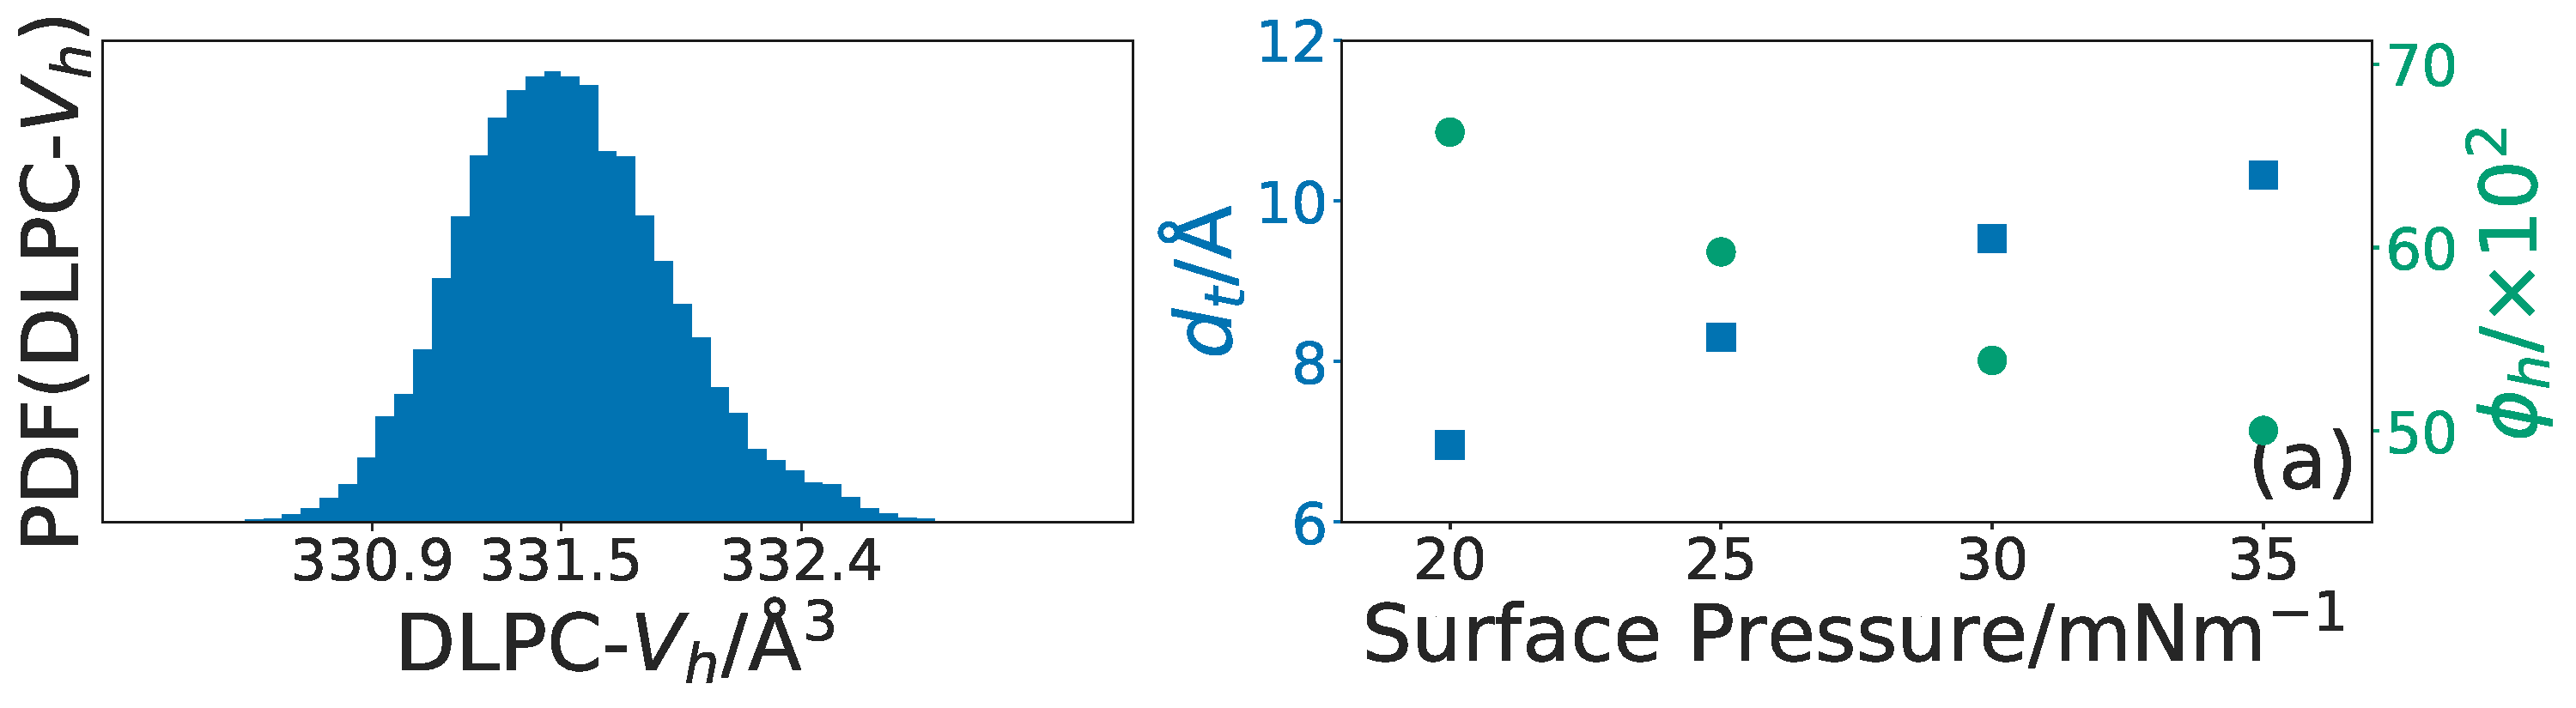
\includegraphics[width=0.48\textwidth]{figures/DLPC_other_data}
	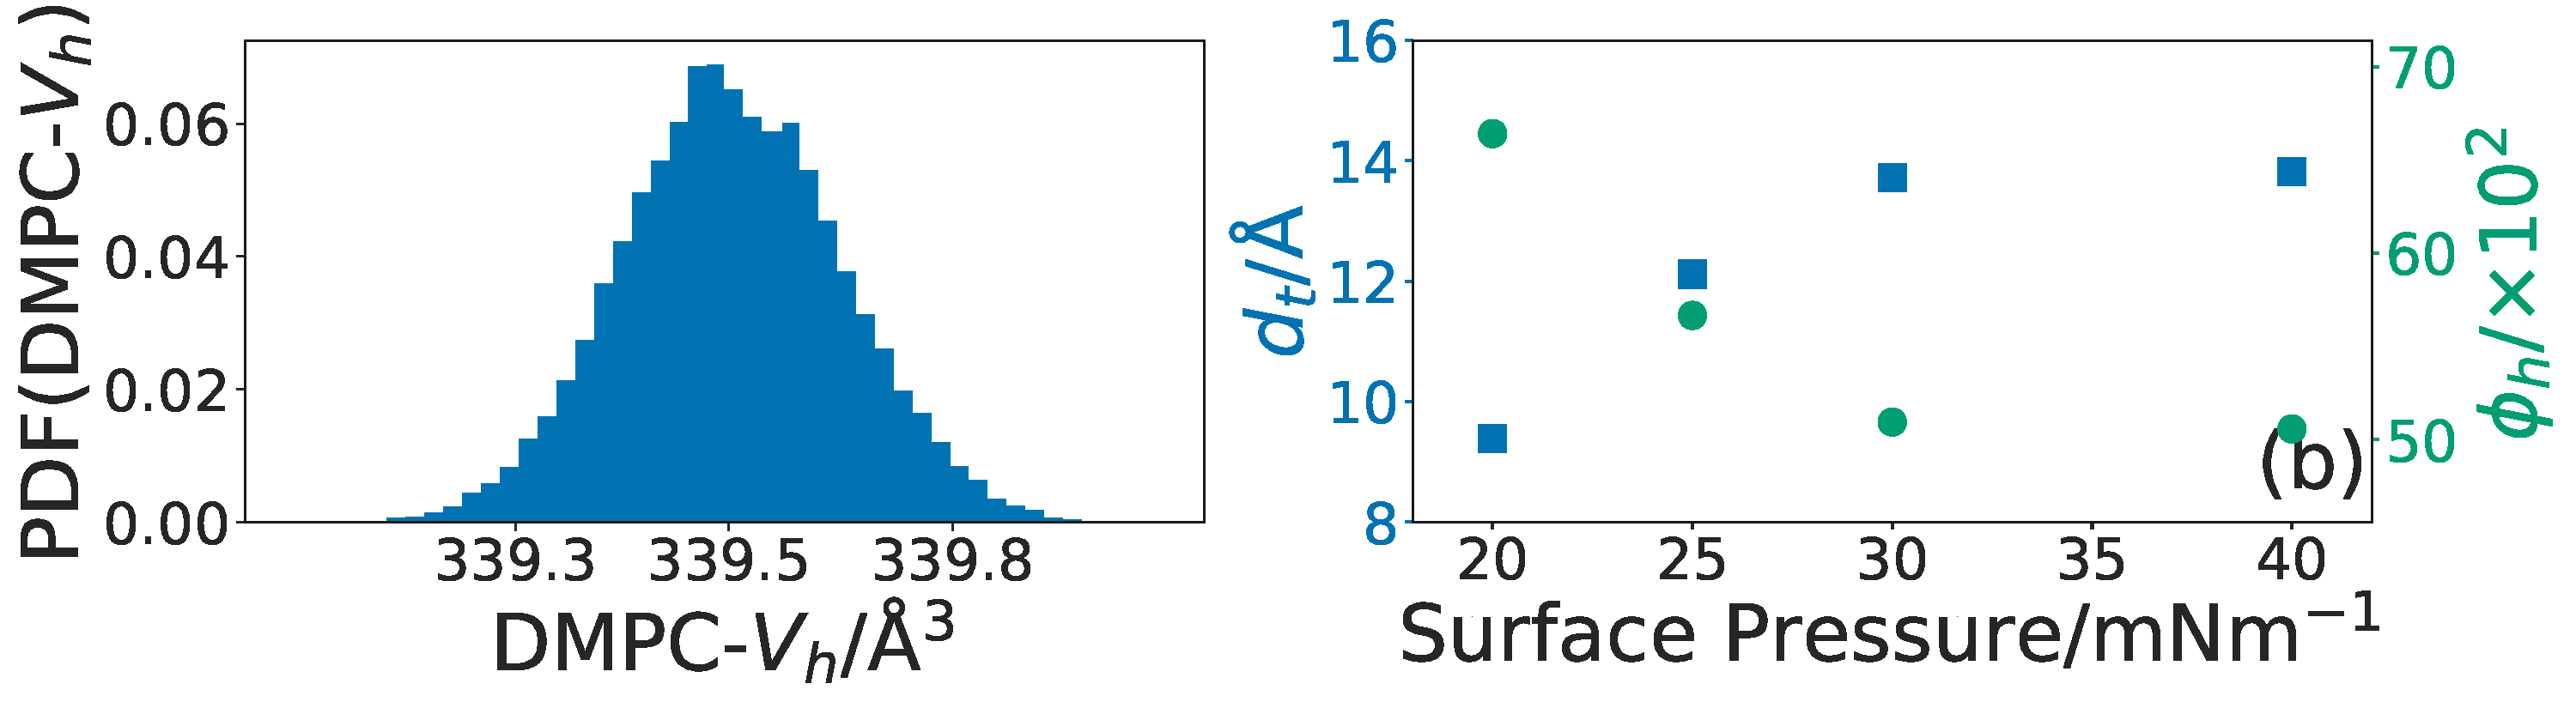
\includegraphics[width=0.48\textwidth]{figures/DMPC_other_data}
	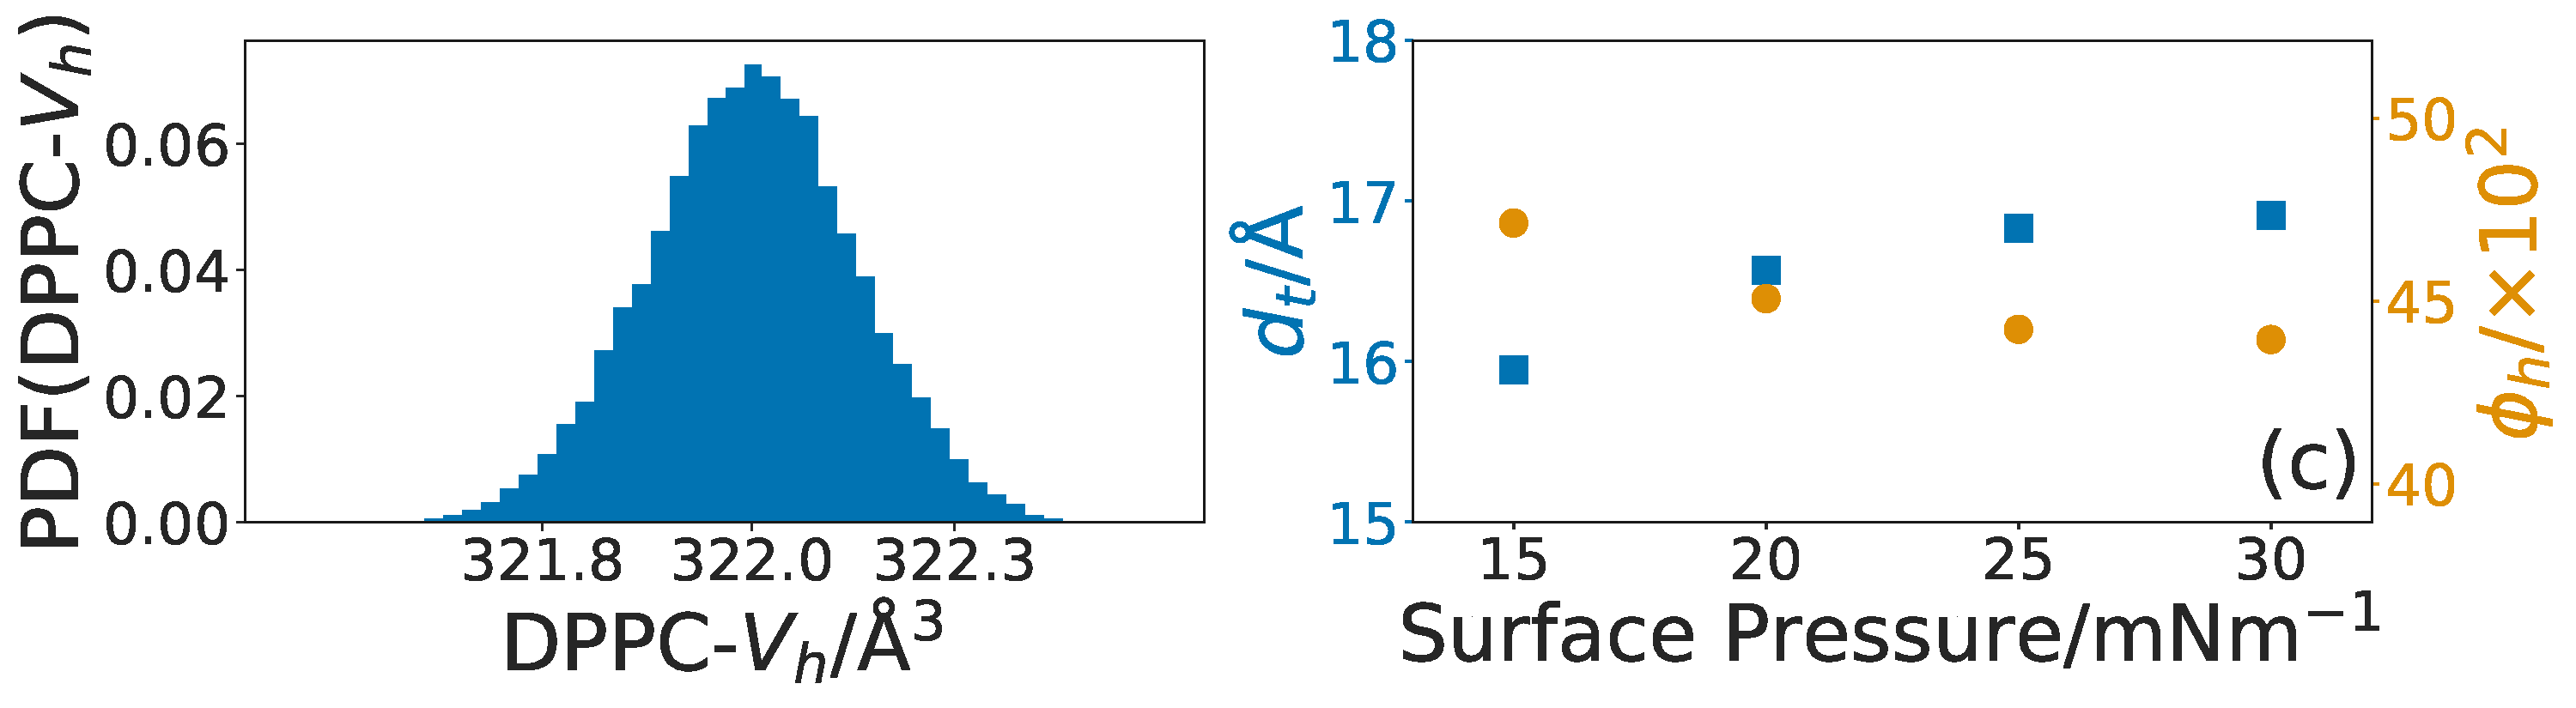
\includegraphics[width=0.48\textwidth]{figures/DPPC_other_data}
	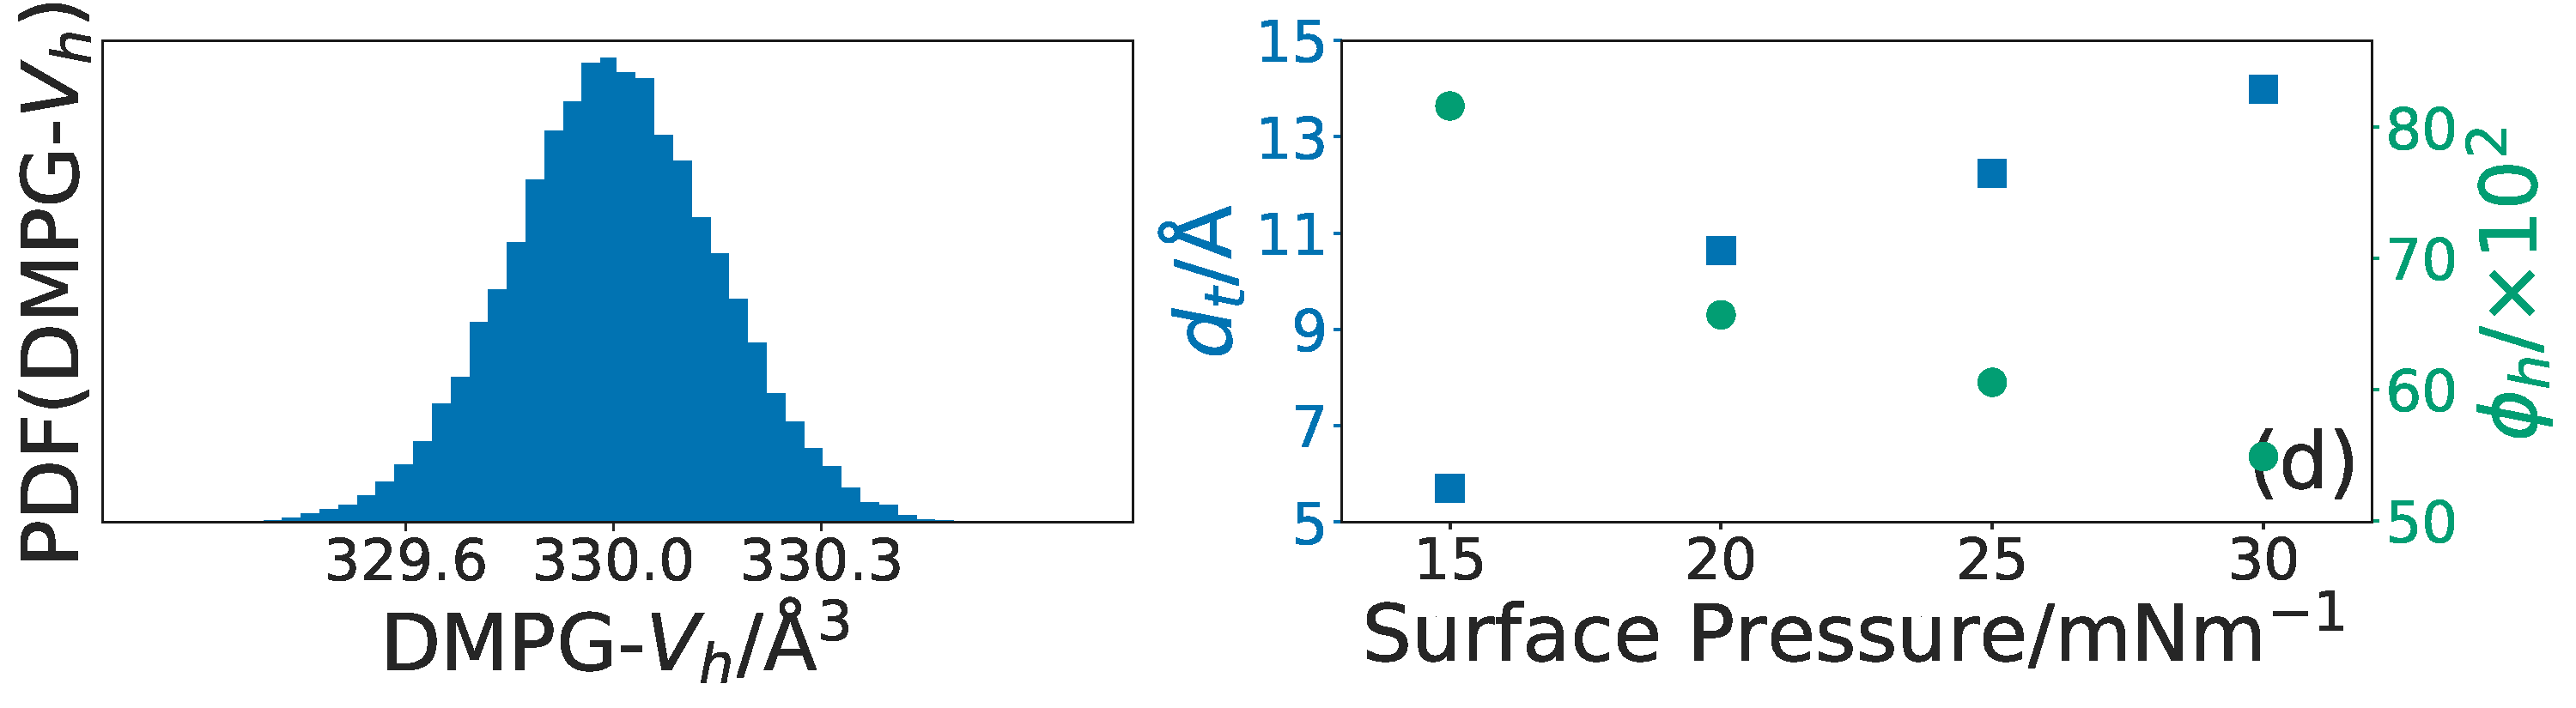
\includegraphics[width=0.48\textwidth]{figures/DMPG_other_data}
	\caption{The PDFs of the head component volume (left) and variation of $d_t$ (blue squares) and $\phi_h$ (green circles) with surface pressure for each of the four lipids; (a) DLPC, (b) DMPC, (c) DPPC, (d) DMPG. Source: Datasets, figure files and running/plotting scripts are available under CC-BY.\cite{mccluskey_2018}}
	\label{fig:lipresults}
\end{figure}
%
The variation of the tail layer thickness in the models, found from $\theta_t$ using Eqn \ref{equ:tl}, with surface pressure is given for each lipid in Figure \ref{fig:lipresults}. It can be observed that as the surface pressure increases, the thickness of the tail layer increases to a point, before plateuing; for DPPC this occurs at 20 mNm$^{-1}$, DMPC at 30 mNm$^{-1}$ and for DMPG and DLPC the plateu can be assumed to be at higher pressures than those studied. This phenomenon of the tail thickness increasing with increasing surface pressure has been noted before for DMPC\cite{Bayerl1990} and DPPC\cite{Campbell2018} at the air-water interface.

\subsection{Effect of compression on solvent concentration}
In Figure \ref{fig:lipresults}, it is clear that for all four lipids, as the surface pressure is increased there is a corresponding decrease in the percentage solvent present in the lipid head layer. This can be rationalised by considering when the surface pressure is increased, the free volume available to the solvent between the lipid head components reduces forcing the solvent out of the lipid head layer and into the bulk. A similar effect has been observed when increasing the surface pressure from 11 mNm$^{-1}$ to 31 mNm$^{-1)}$ for a DMPC/DMPG monolayer at the air-water interface.\cite{Bayerl1990}

\subsection{Effect of compression on the lipid tail component volumes}
It can be seen by comparing Tables \ref{tab:water} and \ref{tab:liptab} that the volume of the lipid tails are significantly lower in the current measurements than found previously, by other techniques. It is unlikely that this is a result of the DES subphase, due to the hydrophobic nature of the lipid tails. However, this reduction observed has been shown previously,\cite{Campbell2018} where it was rationalised by the compaction of the monolayer at elevated surface pressure. In that work, the optimal value of the tail component volume for DPPC was found to be $772$ \AA${^3}$ at a surface pressure of $35$ mNm$^{-1}$, this agrees well with the value of \input{../output/dppc/vt.txt} \AA$^3$ found in this work at surface pressures of 15, 20, 25, and 30 mNm$^{-1}$.

In this work, a single tail component volume was fitted to each lipid for all four surface pressures that were measured. This is based on the assumption, that at all four surface pressures, the lipids adopt the same phase (as discussed in the ESI) and therefore any variation in the structure with surface pressure would manifest only as a change in the tail thickness, via the chain tilt angle. It is clear when comparing Tables \ref{tab:water} and \ref{tab:liptab} that some of the tail component volumes are also reduced in the current XRR measurements compared to those determined previously. The reduction was found to be between 8-12 \% for DPPC, DMPC and DLPC when compared with literature sources at 24-30 $^\circ$C, this is in good agreement with the maximum compression percentage of 15 \% noted by Small and coworkers.\cite{Small1984} DMPG shows a small increase in the tail volume relative to the literature value quoted at lower temperature. Notably our value is similar to that found for DMPC on DES, which has the same tail structure and suggests that our results are at least self-consistent.

\subsection{Solvent effect on lipid head component volumes}
Figure \ref{fig:lipresults} shows the PDFs determined for the head component volume for each of the four lipids. The three lipids with the PC head component are consistent with values of $\sim330$ \AA$^3$, regardless of tail component. This agrees well with the values found for the same head component in water, shown in Table \ref{tab:water}. Interestingly, the component volume for the PG head is similar to that for the PC head with a value of \input{../output/dmpg/vh.txt}\AA$^3$, whereas it is considered to be smaller in water when compared with either DMPG using differential vibrating tube densimetry\cite{Pan2012} or POPG using molecular dynamics simulations.\cite{Kucerka2012} This indicates that there may be some affect arising from the solvation in DES causing an apparent increase in the PG component volume when compared with water.

The major difference between the two head components is the fact PG component is negatively charged whereas the PC component is zwitterionic. It has been shown previously that the conformation for the PC component is folded in water,\cite{Gilliams2016} due to the interaction between the positively-charged ammonium and the negatively-charged phosphate groups. A similar structure may occur for the PG component, with the interaction between the partially postively-charged alcoholic hydrogen atoms and the negatively-charged phosphate group. However, such an interaction would be weaker than that observed in the PC component. Therefore, this observed increase found for the PG component volume in DES when compared with water may be due to the unfolding of the PG head. This unfolding would be made possible by the charged nature of the solvent providing a greater screening effect for the PG head than are present in water. This effect may not be observed for the PC component due to the greater strength of the folding arising from the formally-charged nature of the ammonium group. It would be anticipated that this unfolding would result in an increase in the thickness of the lipid head layer. Previously, DPPG has been reported to have a head layer thickness of $10.3\pm0.4$ \AA\ at 22 mNn$^{-1}$ from neutron reflectometry measurements,\cite{Clifton2012} which it slightly less than the \input{../output/dmpg/head.txt} \AA\ determined in the current work, further suggesting that the unfolding of the PG head component may be occurring as a result of interaction with the DES.

\subsection{Refinement of neutron reflectometry}
The ability to fit the NR data, as shown in Figure \ref{fig:neutron} indicates that the values found for the head component volume is consistant between the pair of measurements for the same system. It is clear, that again stable monolayers of the lipids are forming at the air-DES interface, and that the component volumes determined from XRR measurements are robust-enough to be used in the modelling of NR data. Futhermore, the trends observed with increasing surface pressure in the XRR models, pertaining to the increasing tail thickness and decreasing solvent concentration in the head components are consistant with that found in the NR models.
%
\begin{figure}
	\centering
	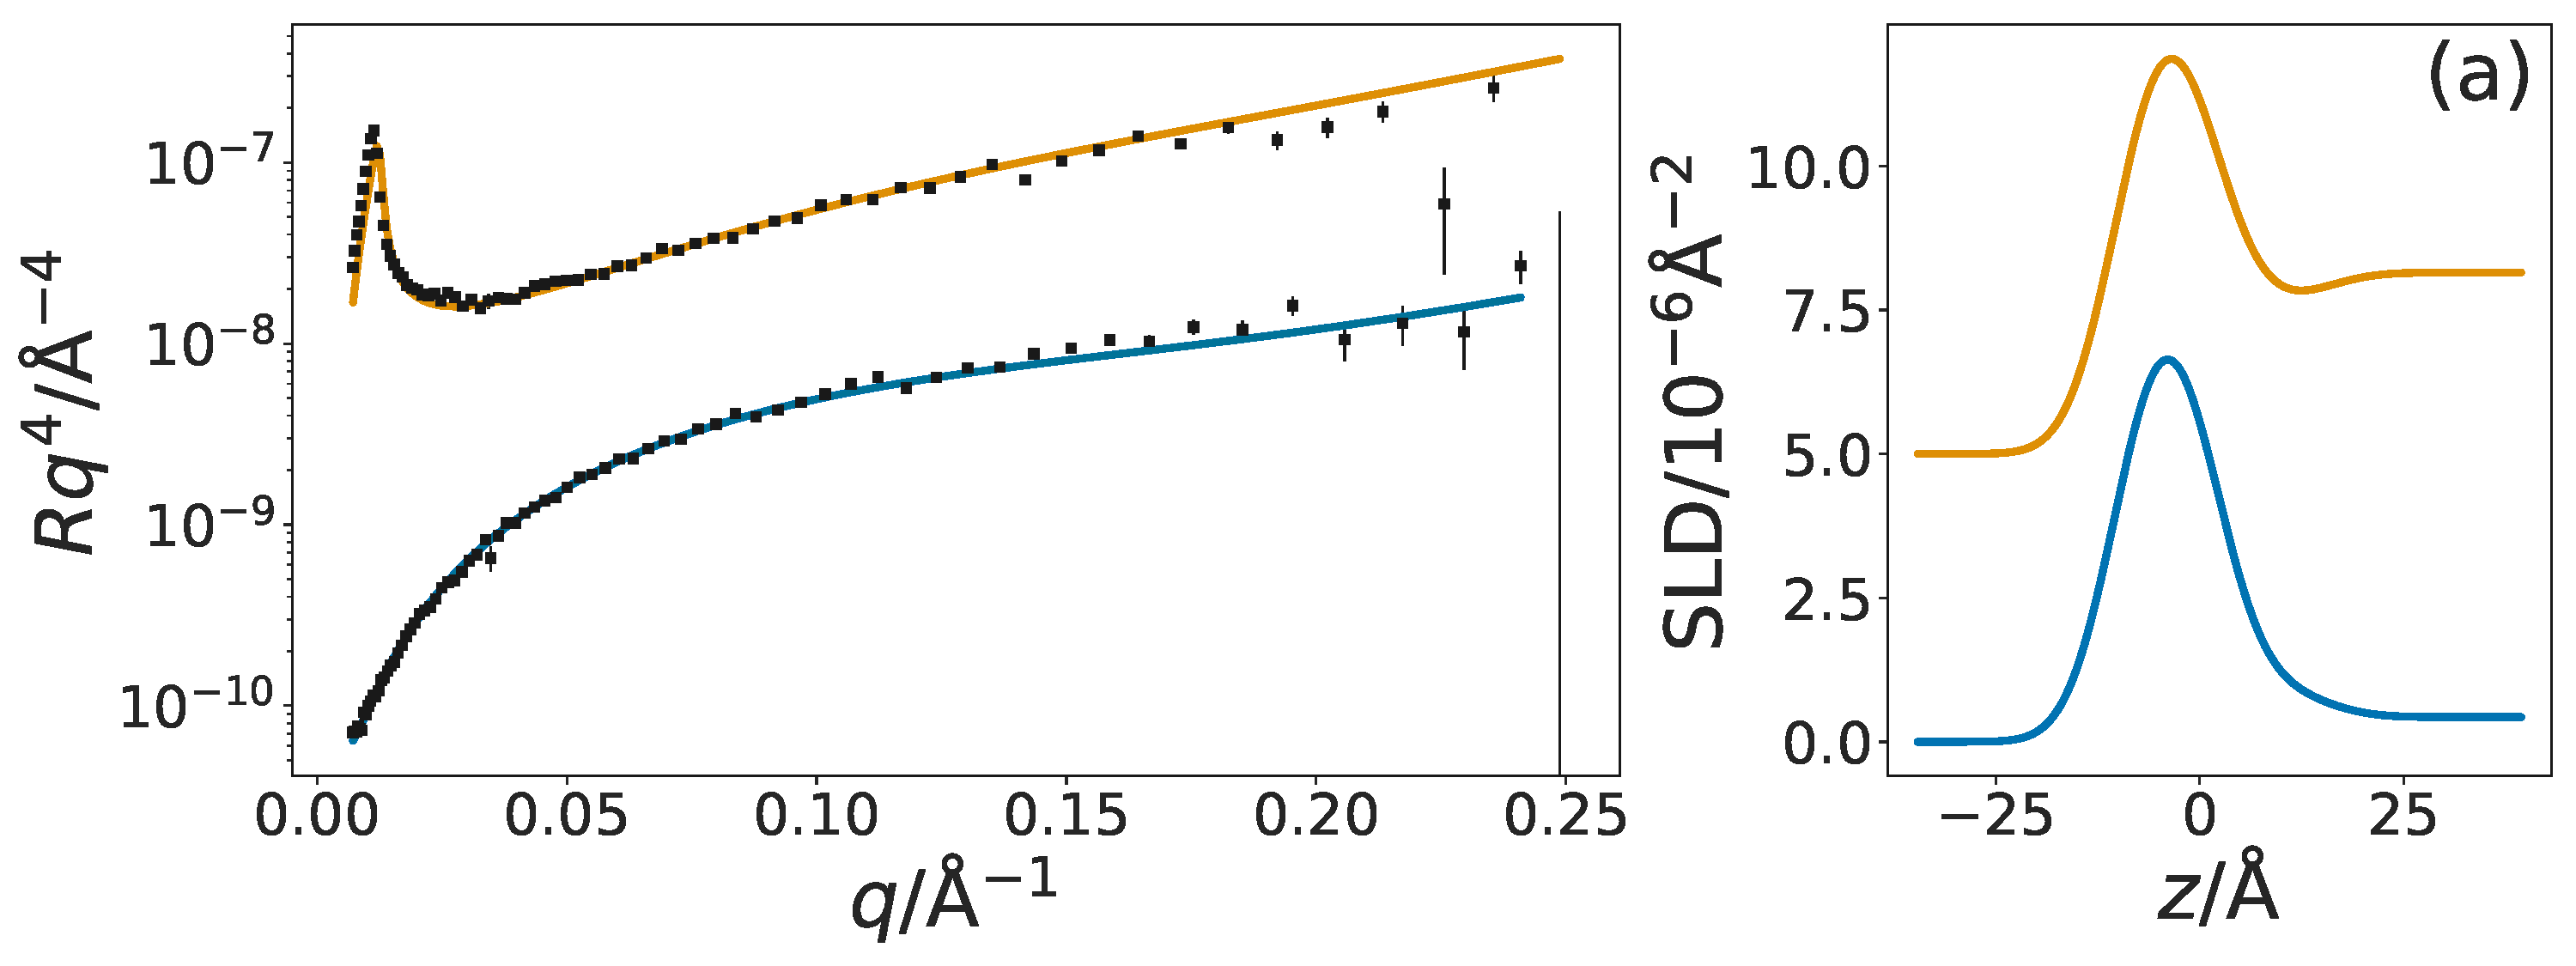
\includegraphics[width=0.48\textwidth]{figures/nDMPC20_all_data}
	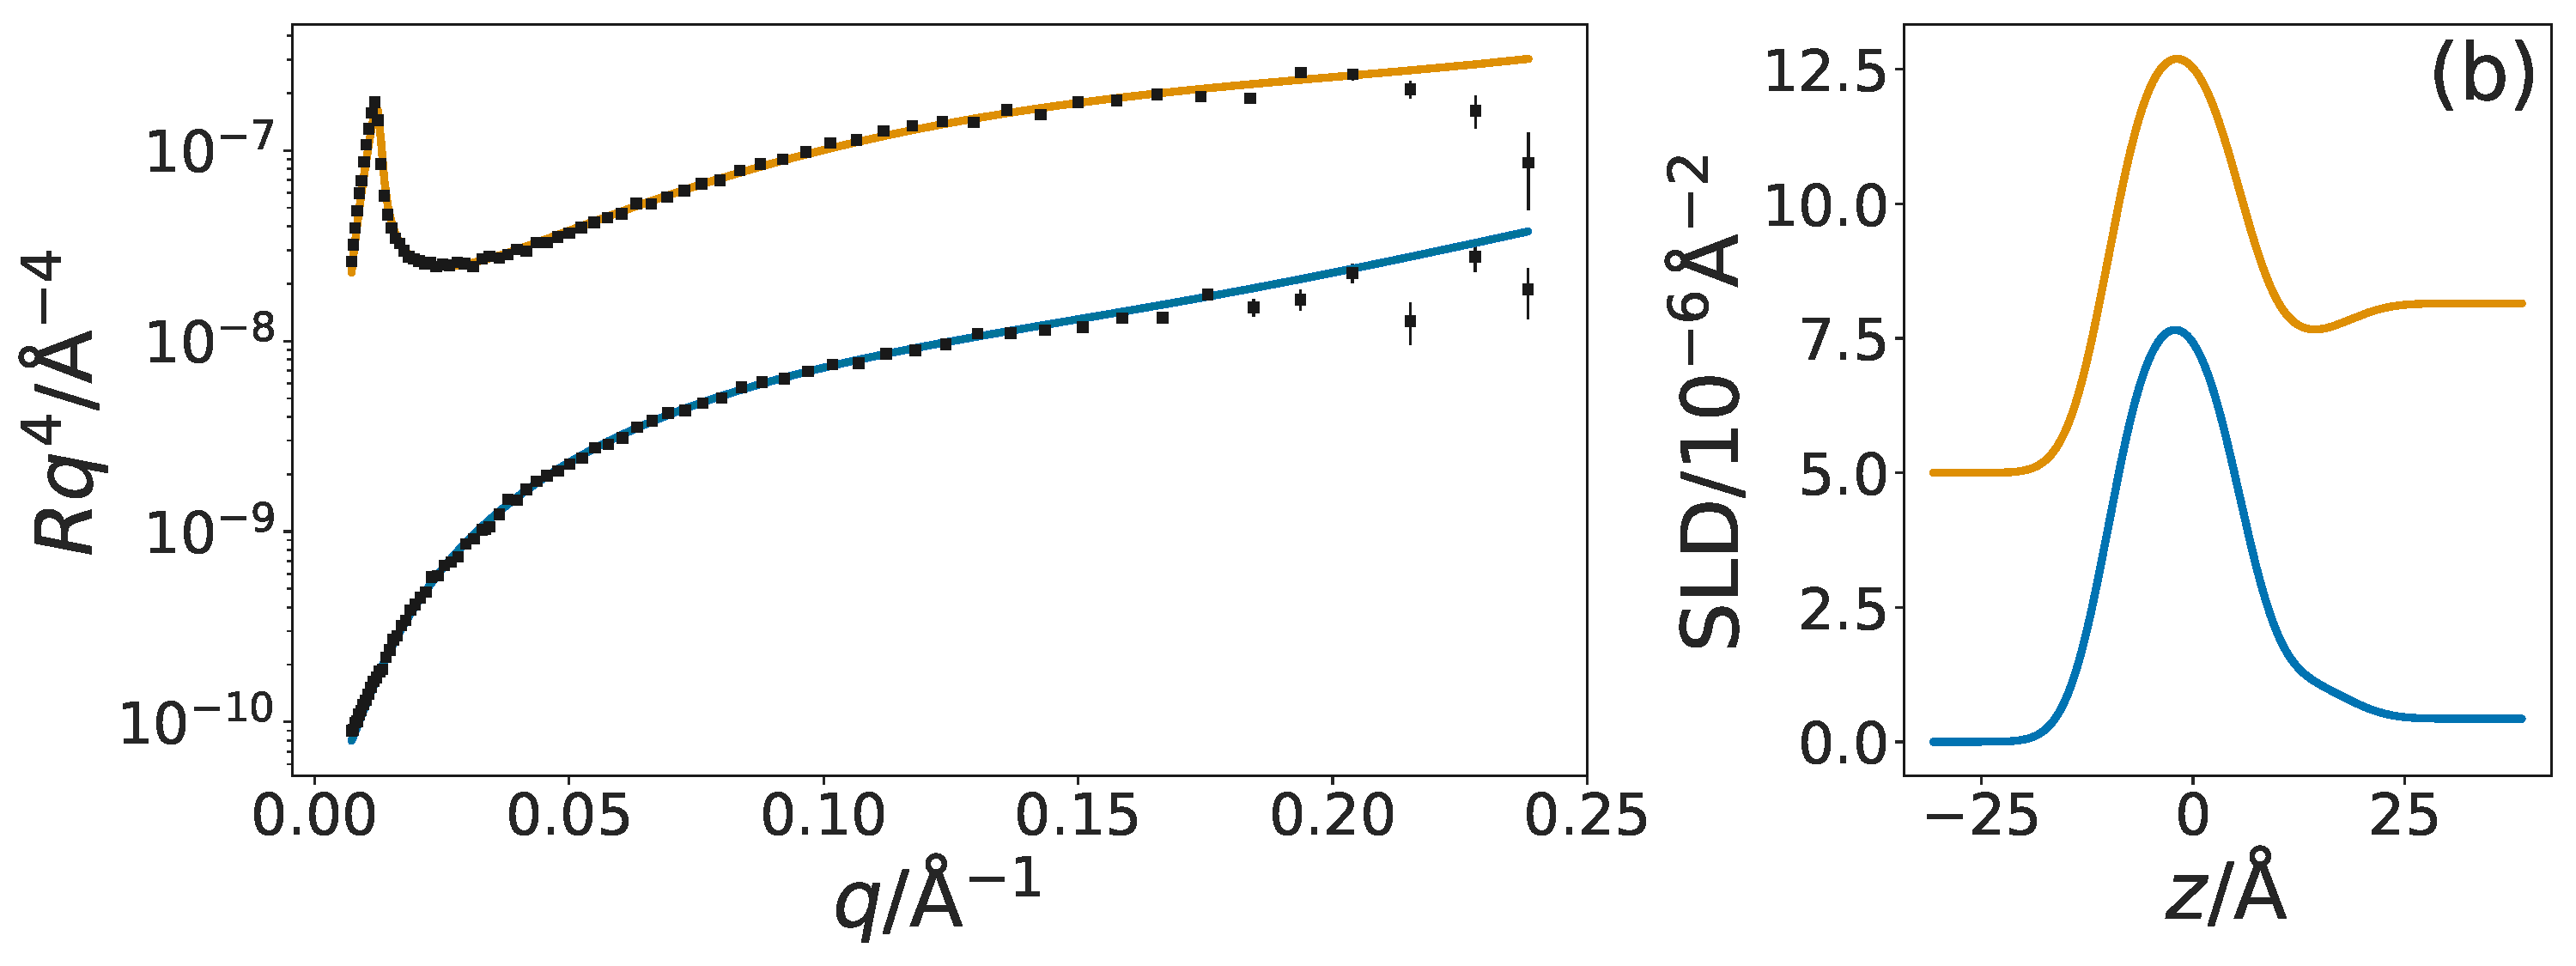
\includegraphics[width=0.48\textwidth]{figures/nDPPC20_all_data}
	\caption{The NR and SLD profiles at a surface pressure of 20 mNm$^{-1}$, the h-DES contrast is shown in blue while the hd-DES in green; (a) DMPC, (b) DPPC. The NR profiles have been offset in the $y$-axis by an order of magnitude and SLD profiles offset in the $y$-axis by $5\times10^{-6}$ \AA$^{-2}$, for clarity. Source: Datasets, figure files and running/plotting scripts are available under CC-BY.\cite{mccluskey_2018}}
	\label{fig:neutron}
\end{figure}
%
\begin{table}
	\small
	\caption{\ The best-fit values, and associated 95 \% confidence intervals for the varying parameters in the co-refined NR models. The values of $d_t$ were found from the appropriate values of $\theta_t$ using Eqn. \ref{equ:tl}, and the values of $\phi_h$ were found using Eqn. \ref{equ:phih}.}
	\label{tab:neutron}
	\begin{tabular*}{0.48\textwidth}{@{\extracolsep{\fill}}lllll}
		\hline
		Lipid & d$_{54}$-DMPC & & d$_{62}$-DPPC & \\
    SP/mNm$^{-1}$ & 20 & 25 & 15 & 20 \\
		\hline
		$\theta_t$/$^\circ$ & \input{../output/dmpc/angle20_neutron.txt} & \input{../output/dmpc/angle25_neutron.txt} & \input{../output/dppc/angle15_neutron.txt} & \input{../output/dppc/angle20_neutron.txt} \\
		$\sigma_{t,h,s}$/\AA & \input{../output/dmpc/rough20_neutron.txt} & \input{../output/dmpc/rough25_neutron.txt} & \input{../output/dppc/rough15_neutron.txt} & \input{../output/dppc/rough20_neutron.txt} \\
    \hline
    $\phi_h$/$\times10^{-2}$ & \input{../output/dmpc/solh20_neutron.txt} & \input{../output/dmpc/solh25_neutron.txt} & \input{../output/dppc/solh15_neutron.txt} & \input{../output/dppc/solh20_neutron.txt} \\
		$d_t$/\AA & \input{../output/dmpc/tail20_neutron.txt} & \input{../output/dmpc/tail25_neutron.txt} & \input{../output/dppc/tail15_neutron.txt} & \input{../output/dppc/tail20_neutron.txt} \\
		\hline
	\end{tabular*}
\end{table}
%

\section{Conclusions}

For the first time, stable phosphocholine and phosphatidylglycerol lipid monolayers have been observed and characterised on a non-aqueous liquid surface. Until the emergence of ionic liquids and DES, only a limited number of molecular solvents exhibited the ability to promote self-assembly and, to the best of our knowledge, only water among those had demonstrated the formation of functional phospholipid monolayers at the air-liquid interface.

A physically and chemically constrained modelling approach and Bayesian analysis method was used to rationalise these measurements showing that the structures are remarkably similar at the air-DES interface to those previously observed at the air-water interface. This has the important implication that DES therefore offer the possibility of performing studies of model membranes in the absence of water. Such applications may include fundamental investigations of phospholipid monolayers in extreme environments (total or partial absence of water, cryogenic temperatures), protein membrane interactions and development of new technologies for drug delivery. However, the fact that the PG component containing lipid did show a significant difference; having a larger head component volume than observed for the same system in water. This that the transfer of lipids to a DES is not just a simple substitution of the subphase. In this specific case we have proposed an explanation based on unfolding of the PG head component that is enabled by electrostatic screening of the component charges by the charged solvent.

The ability to determine the head component volume was facilitated by access to easy to use, and open-source software that allowed for the straightforward use a custom, chemically-consistant model within the analysis of the XRR and NR measurements. Futhermore, this work presents the first, to our knowledge, use of chemically-consistant parameterisation to co-refine XRR measurements at different surface concentrations.

\section*{Conflicts of interest}
There are no conflicts to declare.

\section*{Acknowledgements}
The authors thank the European Spallation Source and the University of Bath Alumni Fund for supporting A.S.-F. A.R.M. is grateful to the University of Bath and Diamond Light Source for co-funding a studentship (Studentship Number STU0149). We also thank Diamond Light Source (SI10546-1) and Institut Laue-Langevin (DOI: \href{http://doi.org/10.5291/ILL-DATA.9-13-612}{10.5291/ILL-DATA.9-13-612}) for the awarded beamtime .

%%%END OF MAIN TEXT%%%

%The \balance command can be used to balance the columns on the final page if desired. It should be placed anywhere within the first column of the last page.

\balance

%If notes are included in your references you can change the title from 'References' to 'Notes and references' using the following command:
%\renewcommand\refname{Notes and references}

%%%REFERENCES%%%
\bibliography{rsc} %You need to replace "rsc" on this line with the name of your .bib file
\bibliographystyle{rsc} %the RSC's .bst file

\end{document}
